%!TEX root =  main.tex
\section{Performance evaluation}
\label{sec:experiments}

In this section, we present the results found for \appname\ with different loads and partitionings and compare them with
\ssmr{}~\cite{bezerra2014ssmr} and \dssmr.
%We are interested in assessing \dssmr{}'s performance with workloads that present different levels of locality.
%By locality, we mean the likelihood that certain groups of data items are accessed together (by the same command).
In Section~\ref{sec:evaluation:setup}, we describe the environment where we conducted our experiments.
In Section~\ref{sec:evaluation:strongloc}, we show the results.

% with strong-locality workloads.
%In Section~\ref{sec:evaluation:weakloc}, we show the results for weak-locality workloads.

%\begin{figure*}
%\begin{minipage}[b]{1\linewidth} % A minipage that covers the whole width of the page
%\centering
%      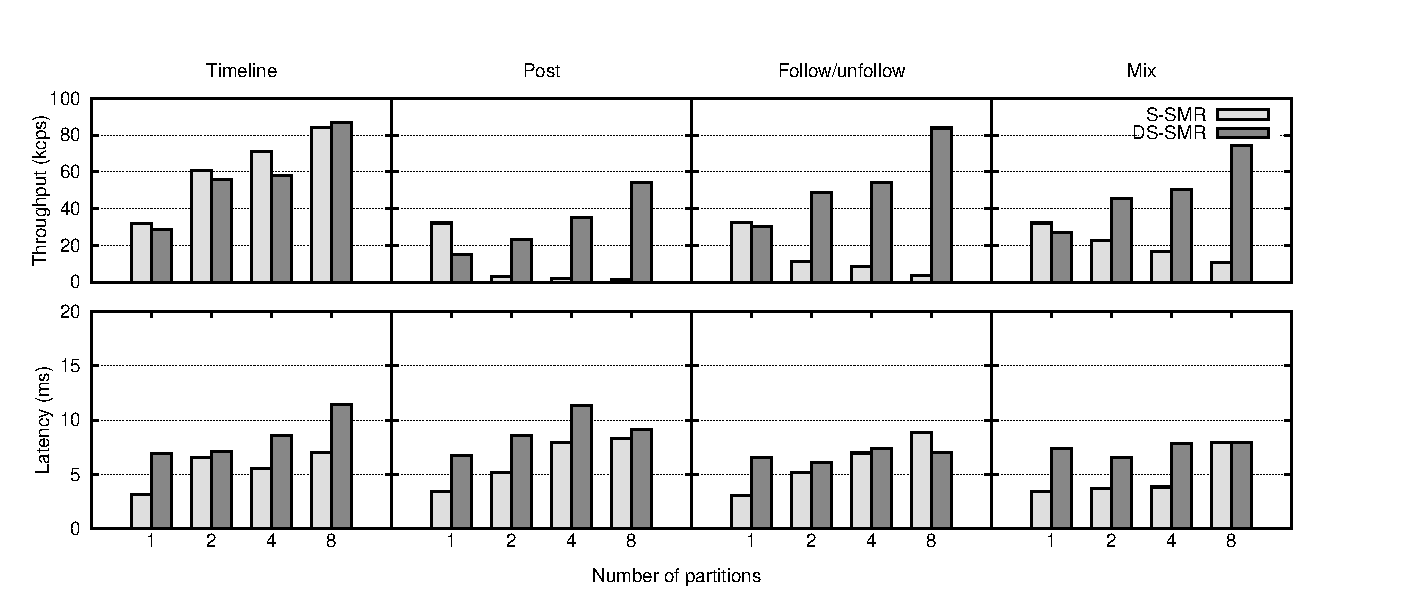
\includegraphics[width=1.08\linewidth]{figures/graphs/strong-locality}
%\end{minipage}
%\caption{Results of \appname\ running with \ssmr\ and \dssmr{}. Throughput is shown in thousands of commands per second (kcps).}
%\label{fig:strongloc}
%\end{figure*}
%\begin{table*}[htp]
%\vspace{10mm}
%\caption{Absolute values of \appname\ running \ssmr\ and \dssmr{}.}
%\centering
%\begin{adjustbox}{max width=\textwidth}
%\begin{tabular}{|l|c|c|c|c|c|c|c|c|c|c|c|c|c|c|c|c|} \hline
%         & \multicolumn{4}{|c|}{Timeline}  &  \multicolumn{4}{|c|}{Post}   &  \multicolumn{4}{|c|}{Follow/unfollow}  &  \multicolumn{4}{|c|}{Mix}    \\ \hline
%         & 1     & 2     & 4     & 8       & 1     & 2     & 4   & 8    & 1     & 2     & 4       & 8           & 1     & 2     & 4     & 8     \\ \hline\hline
%         & \multicolumn{16}{|c|}{Throughput (commands per second)} \\ \hline
%\ssmr\   & 31757 & 60699 & 71274 & 84065   & 32151 & 2884  & 1894  & 1200  & 32541 & 11476 & 8580    & 3371          & 32151 & 22803 & 16822 & 10657 \\ \hline
%\dssmr\  & 28882 & 55925 & 57900 & 86685   & 14874 & 23295 & 35188 & 54250 & 30215 & 48976 & 54025   & 83880         & 27101 & 45686 & 50671 & 74257 \\ \hline\hline
%         & \multicolumn{16}{|c|}{\textbf{Throughput rate = \dssmr\ tput / \ssmr\ tput}} \\ \hline
%         & \textbf{0.91} & \textbf{0.92}  & \textbf{0.81} & \textbf{1.03}     & \textbf{0.46}   & \textbf{8.08}   & \textbf{18.48}  & \textbf{45.00} & \textbf{0.93} & \textbf{4.27} & \textbf{6.30} & \textbf{24.88} & \textbf{0.84} & \textbf{2.00} & \textbf{3.01} & \textbf{6.97} \\ \hline\hline
%         & \multicolumn{16}{|c|}{Latency (milliseconds)} \\ \hline
%\ssmr\   & 3.1 & 6.6 & 5.6 & 7.0  & 3.4 & 5.2  & 7.9  & 8.3  & 3.0  & 5.2  & 7.0  & 8.8  & 3.4  & 3.7  & 3.8  & 7.9  \\ \hline
%\dssmr\  & 6.9 & 7.1 & 8.6 & 11.4 & 6.7 & 8.6  & 11.3 & 9.1  & 6.6  & 6.1  & 7.4  & 7.0  & 7.3  & 6.5  & 7.8  & 7.9  \\ \hline
%\end{tabular}
%\end{adjustbox}
%\label{tbl:results}
%\vspace{10mm}
%\end{table*}%

\subsection{Environment setup and configuration parameters}
\label{sec:evaluation:setup}

We conducted all experiments on a cluster that had two types of nodes: (a) HP SE1102 nodes, equipped with two Intel Xeon L5420 processors running at 2.5 GHz and with 8 GB of main memory, and (b) Dell SC1435 nodes, equipped with two AMD Opteron 2212 processors running at 2.0 GHz and with 4 GB of main memory. The HP nodes were connected to an HP ProCurve 2920-48G gigabit network switch, and the Dell nodes were connected to another, identical switch. Those switches were interconnected by a 20 Gbps link.
All nodes ran CentOS Linux 7.1 with kernel 3.10 and had the OpenJDK Runtime Environment~8 with the \mbox{64-Bit} Server VM (build 25.45-b02).
%We kept the clocks synchronized using NTP in order to measure latency components involving events in different computers.

For the experiments, we use the following workloads:
Timeline (composed only of getTimeline requests),
Post (only post requests),
Follow/unfollow (50\% of follow requests and 50\% of unfollow), and
Mix (7.5\% post, 3.75\% follow, 3.75\% unfollow, and 85\% getTimeline).

\subsection{Methodology and goals}
All static graphs were generated using the Holme-Kim model \cite{holme-kim}, it generates power-law graphs
with a clustering coefficient, such graphs, also referred as scale-free, are a good representation
of the geometric structure of social networks.

In the experiments, we tested graphs with 10.000 users with a varying percentage of edge-cuts, to get the desired edge-cut
percentage, we run METIS partitioner for each partitioning size. METIS performs well in graphs with less than 10 million nodes, and scales linearly as seen in Figure~\ref{fig:metis_size_time}, with both memory and cpu usage.

\begin{figure}[t]
	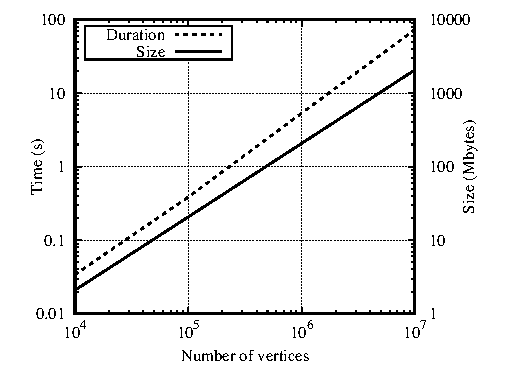
\includegraphics[width=0.95\columnwidth]{figures/metis_size_time}
	\caption{METIS processor and memory usage}
	\label{fig:metis_size_time}
\end{figure}


\subsection{Results}




\label{sec:evaluation:strongloc}

